
\chapter[Các định luật bảo toàn\\ trong phản ứng hạt nhân]{Các định luật bảo toàn trong phản ứng hạt nhân}
\section{Lý thuyết}

\subsection{Các định luật bảo toàn trong phản ứng hạt nhân}
Xét phản ứng hạt nhân
\begin{equation}
	^{A_1}_{Z_1}A + ^{A_2}_{Z_2}B \rightarrow ^{A_3}_{Z_3}C + ^{A_4}_{Z_4}D
\end{equation}
\subsubsection{Định luật bảo toàn điện tích}
Trong phản ứng hạt nhân, tổng đại số điện tích các hạt tương tác bằng tổng đại số điện tích các hạt sản phẩm
\begin{equation}
	Z_1+Z_2=Z_3+Z_4.
\end{equation}
\subsubsection{Định luật bảo toàn số khối}
Trong phản ứng hạt nhân, tổng số nuclon các hạt tương tác bằng tổng số nuclon các hạt sản phẩm
\begin{equation}
	A_1+A_2=A_3+A_4.
\end{equation}

\subsubsection{Định luật bảo toàn năng lượng toàn phần}
Năng lượng toàn phần bao gồm động năng và năng lượng nghỉ. Trong phản ứng hạt nhân, tổng năng lượng toàn phần của các hạt bằng tổng năng lượng toàn phần của các hạt sản phẩm
\begin{equation}
	E_A+E_B=E_C+E_D
\end{equation}
\begin{equation}
	\Leftrightarrow m_Ac^2+ W_{\textrm{đ }A} + m_Bc^2+W_{\textrm{đ }B} = m_Cc^2+ W_{\textrm{đ }C} + m_Dc^2+W_{\textrm{đ }D}
\end{equation}
\begin{equation}
	\Leftrightarrow W_\textrm{đ trước} + (m_A+m_B)c^2 = W_\textrm{đ sau} + (m_C+m_D)c^2 .
\end{equation}

\subsubsection{Định luật bảo toàn động lượng}
Trong phản ứng hạt nhân, vectơ tổng động lượng của các hạt tương tác bằng vectơ tổng động lượng của các hạt sản phẩm.
\begin{equation}
	\vec{p}_A + \vec{p}_B = \vec{p}_C + \vec{p}_D
\end{equation}
\begin{equation}
	\Leftrightarrow m_A\vec{v}_A + m_B\vec{v}_B = m_C\vec{v}_C + m_D\vec{v}_D.
\end{equation}

\subsection{Năng lượng tỏa ra hay thu vào trong phản ứng hạt nhân}
Do tính chất không bảo toàn khối lượng nghỉ, nhưng lại bảo toàn năng lượng toàn phần của hệ trong phản ứng hạt nhân, nên các phản ứng hạt nhân có thể tỏa ra năng lượng hoặc thu vào năng lượng. 

Gọi $m_\text{trước}$ là tổng khối lượng nghỉ của các hạt trước phản ứng và $m_\text{sau}$ là tổng khối lượng nghỉ của các hạt sau phản ứng. Năng lượng của một phản ứng hạt nhân là
\begin{equation}
	\Delta W = \left(m_\text{trước} - m_\text{sau}\right) c^2;
\end{equation}
trong đó:
\begin{itemize}
	\item Nếu $m_\text{trước}$ > $m_\text{sau} \Rightarrow \Delta W >0$ thì phản ứng tỏa năng lượng;
	\item Nếu $m_\text{trước}$ < $m_\text{sau} \Rightarrow \Delta W < 0$ thì phản ứng thu năng lượng.
\end{itemize}

%	\manatip{\textbf{Dư tỏa nợ thu} (Dương tỏa âm thu - Ngược lại với cân bằng hóa học).}

\section{Mục tiêu bài học - Ví dụ minh họa}

\begin{dang}{Năng lượng phản ứng, nhiên liệu cần đốt.}
	
	\ppgiai{
		
		Xét phản ứng hạt nhân
		\begin{equation*}
			^{A_1}_{Z_1}A + ^{A_2}_{Z_2}B \rightarrow ^{A_3}_{Z_3}C + ^{A_4}_{Z_4}D
		\end{equation*}
		
		Năng lượng của phản ứng hạt nhân có thể tính theo các công thức sau:
		\begin{itemize}
			\item Tính theo khối lượng
			\begin{equation*}
				\Delta W = \left(m_\text{trước} - m_\text{sau}\right) c^2;
			\end{equation*}
			\begin{equation*}
				\Leftrightarrow \Delta W = \left[ \left(m_A + m_B\right)  - \left( m_C + m_D\right)\right]  c^2;
			\end{equation*}
			trong đó: $m_A$, $m_B$, $m_C$, $m_D$ lần lượt là khối lượng nghỉ của các hạt nhân $X_A$, $X_B$, $X_C$, $X_D$.
			
			\item Tính theo độ hụt khối
			\begin{equation*}
				\Delta W = \left(\Delta m_\text{sau} - \Delta m_\text{trước}\right) c^2;
			\end{equation*}
			\begin{equation*}
				\Leftrightarrow \Delta W = \left[\left(\Delta m_C + \Delta m_D \right) -  \left(\Delta m_A + \Delta m_B\right)\right] c^2;
			\end{equation*}
			trong đó: $\Delta m_A$, $\Delta m_B$, $\Delta m_C$, $\Delta m_D$ lần lượt là độ hụt khối của các hạt nhân $X_A$, $X_B$, $X_C$, $X_D$.
			
			\item Tính theo năng lượng liên kết, năng lượng liên kết riêng
			\begin{equation*}
				\Delta W = \left(W_\text{lk sau} - W_\text{lk trước}\right) c^2;
			\end{equation*}
			\begin{equation*}
				\Leftrightarrow \Delta W = \left[\left(W_{\textrm{lk }C} + W_{\textrm{lk }D} \right) -  \left(W_{\textrm{lk }A} + W_{\textrm{lk }B}\right)\right] c^2;
			\end{equation*}
			\begin{equation*}
				\Leftrightarrow \Delta W = \left[\left(A_C\cdot W_{\textrm{lkr }C} + A_D\cdot W_{\textrm{lkr }D} \right) -  \left(A_A\cdot W_{\textrm{lkr }A} + A_B\cdot W_{\textrm{lkr }B}\right)\right] c^2;
			\end{equation*}
			trong đó:
			\begin{itemize}
				\item $W_{\textrm{lk }A}$, $W_{\textrm{lk }B}$, $W_{\textrm{lk }C}$, $W_{\textrm{lk }D}$ lần lượt là năng lượng liên kết của các hạt nhân $X_A$, $X_B$, $X_C$, $X_D$.
				
				\item $W_{\textrm{lkr }A}$, $W_{\textrm{lkr }B}$, $W_{\textrm{lkr }C}$, $W_{\textrm{lkr }D}$ lần lượt là năng lượng liên kết riêng của các hạt nhân $X_A$, $X_B$, $X_C$, $X_D$.
				
				\item $A_A$, $A_B$, $A_C$, $A_D$ lần lượt là số khối của các hạt nhân $X_A$, $X_B$, $X_C$, $X_D$.
			\end{itemize}
			
			\item Tính theo động năng
			\begin{equation*}
				\Delta W = \left(W_\textrm{đ sau} - W_\textrm{đ trước}\right) c^2;
			\end{equation*}
			\begin{equation*}
				\Leftrightarrow \Delta W = \left[ \left(W_{\textrm{đ }C} + W_{\textrm{đ }D}\right)  - \left( W_{\textrm{đ }A} + W_{\textrm{đ }B}\right)\right]  c^2;
			\end{equation*}
			trong đó: $W_{\textrm{đ }A}$, $W_{\textrm{đ }B}$, $W_{\textrm{đ }C}$, $W_{\textrm{đ }D}$ lần lượt là động năng của các hạt nhân $X_A$, $X_B$, $X_C$, $X_D$.
	\end{itemize}}
	
	\luuy{
		Năng lượng tương ứng với khối lượng $\SI{1}{u}$ được xác định
		\begin{equation*}
			\SI{1}{\atomicmassunit}\cdot c^2=\SI{931,5}{\mega\electronvolt}.
		\end{equation*}
	}
	
	\viduii{2}
	{
		[THPT QG 2017 - Mã đề 206] Trong một phản ứng hạt nhân, tổng khối lượng nghỉ của các hạt trước phản ứng là $\SI{37,9638}{u}$ và tổng khối lượng nghỉ các hạt sau phản ứng là  $\SI{37,9656}{u}$. Lấy $\SI{1}{u}=\SI{931,5}{\mega\electronvolt/c^2}$ . Phản ứng này
		
		\begin{mcq}(2)
			\item tỏa năng lượng $\SI{1,68}{\mega\electronvolt}$.
			\item thu năng lượng $\SI{1,68}{\mega\electronvolt}$.
			\item thu năng lượng $\SI{16,8}{\mega\electronvolt}$.
			\item tỏa năng lượng $\SI{16,8}{\mega\electronvolt}$.
	\end{mcq}}
	{
		\begin{center}
			\textbf{Hướng dẫn giải}
		\end{center}
		
		Năng lượng của phản ứng hạt nhân là
		\begin{eqnarray*}
			\Delta W &=& \left(m_\text{trước} - m_\text{sau}\right) c^2 \\
			&=& \left(\SI{37,9638}{u} - \SI{37,9656}{u}\right) c^2\\
			&=&\left(\SI{37,9638}{} - \SI{37,9656}{}\right) \text{u}c^2\\
			&=&\left(\SI{37,9638}{} - \SI{37,9656}{}\right) \cdot\SI{931,5}{\mega\electronvolt/c^2}\cdot c^2\\
			&=&-\SI{1,68}{\mega\electronvolt}.
		\end{eqnarray*}
		
		Vì $\Delta W = -\SI{1,68}{\mega\electronvolt} < 0$ nên phản ứng thu năng lượng $\SI{1,68}{\mega\electronvolt}$.
		
		\begin{center}
			\textbf{Câu hỏi tương tự}
		\end{center}
		
		Giả sử trong một phản ứng hạt nhân, tổng khối lương hai hạt trước phản ứng lớn hơn tổng khối lượng hai hạt sau phản ứng là $\SI{0.02}{u}$. Cho $\SI{1}{u} = \SI{931.5}{MeV/c^2}$. Phản ứng hạt nhân này
		\begin{mcq}(2)
			\item tỏa năng lượng $\SI{1.863}{MeV}$.
			\item thu năng lượng $\SI{1.863}{MeV}$.
			\item tỏa năng lượng $\SI{18.63}{MeV}$.
			\item thu năng lượng $\SI{18.63}{MeV}$.
		\end{mcq}
		
		\textbf{Đáp án:} C.
	}
	\viduii{2}
	{
		[Đề thi đại học khối A năm 2009] Cho phản ứng hạt nhân $^3_1\text{T} + ^2_1 \text{D} \rightarrow ^4_2\text{He} + X$. Lấy độ hụt khối của hạt nhân $\text{T}$, hạt nhân $\text{D}$, hạt $\text{He}$ lần lượt là $\SI{0,009106}{u}$; $\SI{0,002491}{u}$; $\SI{0,030382}{u}$ và $\SI{1}{u}=\SI{931,5}{\mega\electronvolt/c^2}$. Năng lượng tỏa ra của phản ứng xấp xỉ bằng
		
		\begin{mcq}(2)
			\item $\SI{15,017}{\mega\electronvolt}$.
			\item $\SI{200,025}{\mega\electronvolt}$.
			\item $\SI{17,498}{\mega\electronvolt}$.
			\item $\SI{21,076}{\mega\electronvolt}$.
		\end{mcq}
	}
	{\begin{center}
			\textbf{Hướng dẫn giải}
		\end{center}
		
		Năng lượng của phản ứng hạt nhân là
		
		\begin{eqnarray*}
			\Delta W &=& \left(\Delta m_\text{sau} - \Delta m_\text{trước}\right) c^2 \\
			&=& \left[\left(\Delta m_\text{He} + \Delta m_\text{X} \right) -  \left(\Delta m_\text{T} + \Delta m_\text{D}\right)\right] c^2\\
			&=& \left[\left(\SI{0,030382}{u} + 0 \right) -  \left(\SI{0,009106}{u} + \SI{0,002491}{u}\right)\right] c^2\\
			&=& \left[\left(\SI{0,030382}{} \right) -  \left(\SI{0,009106}{} + \SI{0,002491}{}\right)\right] \text{u} c^2\\
			&=& \left[\SI{0,030382}{}  -  \left(\SI{0,009106}{} + \SI{0,002491}{}\right)\right] \cdot\SI{931,5}{\mega\electronvolt/c^2}\cdot c^2\\
			&=&\SI{17,498}{\mega\electronvolt}.
		\end{eqnarray*}
		
		\begin{center}
			\textbf{Câu hỏi tương tự}
		\end{center}
		
		Cho phản ứng hạt nhân $^{23}_{11} \text{Na} + ^{1}_{1} \text{H} \longrightarrow ^{4}_{2} \text{He} + ^{20}_{10} \text{Ne}$. Lấy khối lượng của các hạt nhân $^{23}_{11} \text{Na}$, $^{20}_{10} \text{Ne}$, $^{4}_{2} \text{He}$, $^{1}_{1} \text{H}$ lần lượt là $\SI{22.9837}{u}$, $\SI{19.9869}{u}$, $\SI{4.0015}{u}$, $\SI{1.0073}{u}$ và $\SI{1}{u} = \SI{931.5}{MeV/c^2}$. Năng lượng của phản ứng này
		\begin{mcq}(2)
			\item thu vào $\SI{2.4219}{MeV}$.
			\item thu vào $\SI{3.4524}{MeV}$.
			\item tỏa ra $\SI{3.4524}{MeV}$.
			\item tỏa ra $\SI{2.4219}{MeV}$.
		\end{mcq}
		\textbf{Đáp án:} D.
	}
	
\end{dang}

\begin{dang}{Động năng, động lượng, vận tốc,\\ góc tạo bởi các hạt.}
	
	\ppgiai{
		Xét phản ứng hạt nhân
		\begin{equation*}
			^{A_1}_{Z_1}A + ^{A_2}_{Z_2}B \rightarrow ^{A_3}_{Z_3}C + ^{A_4}_{Z_4}D
		\end{equation*}
		\begin{description}
			\item[Bước 1:] Viết phương trình định luật bảo toàn động lượng
			\begin{equation*}
				\vec{p}_A + \vec{p}_B = \vec{p}_C + \vec{p}_D
			\end{equation*}
			\begin{equation*}
				\Leftrightarrow m_A\vec{v}_A + m_B\vec{v}_B = m_C\vec{v}_C + m_D\vec{v}_D.
			\end{equation*}
			\item[Bước 2:] Viết phương trình định luật bảo toàn năng lượng toàn phần
			\begin{equation*}
				E_A+E_B=E_C+E_D
			\end{equation*}
			\begin{equation*}
				\Leftrightarrow m_Ac^2+ W_{\textrm{đ }A} + m_Bc^2+W_{\textrm{đ }B} = m_Cc^2+ W_{\textrm{đ }C} + m_Dc^2+W_{\textrm{đ }D}
			\end{equation*}
			\begin{equation*}
				\Leftrightarrow W_\textrm{đ trước} + (m_A+m_B)c^2 = W_\textrm{đ sau} + (m_C+m_D)c^2 .
			\end{equation*}
			
			\item[Bước 3:] Giải hệ phương trình ở bước 1 và bước 2.
	\end{description}}
	\luuy{
		Mối liên hệ giữa động lượng $p$ và động năng $W_\text{đ}$ là
		\begin{equation*}
			p=\sqrt{2mW_\text{đ}}\textrm{ hoặc }W_\text{đ}=\dfrac{p^2}{2m}.
		\end{equation*}
	}
	
	\viduii{3}
	{
		[Đề thi đại học năm 2011] Bắn một proton vào hạt nhân $^7_3\text{Li}$ đứng yên. Phản ứng tạo ra hai hạt nhân $X$ giống nhau bay ra với cùng tốc độ theo các phương hợp với phương tới của proton các góc bằng nhau là $60^\circ$. Lấy khối lượng của mỗi hạt nhân tính theo đơn vị u bằng số khối của nó. Tỉ số giữa tốc độ của prôtôn và tốc độ của hạt nhân $X$ là
		
		\begin{mcq}(4)
			\item 4.
			\item $\dfrac{1}{4}$.
			\item 2.
			\item $\dfrac{1}{2}$.
	\end{mcq}}
	{
		\begin{center}
			\textbf{Hướng dẫn giải}
		\end{center}
		
		\begin{center}
			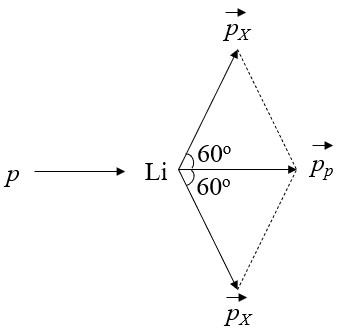
\includegraphics[scale=0.8]{../figs/VN12-PH-47-L-028-2-H1.jpg}
		\end{center}
		
		Phương trình phản ứng:
		\begin{equation*}
			^1_1 p + ^7_3\text{Li} \rightarrow 2 ^4_2 X
		\end{equation*}
		
		Áp dụng định luật toàn động lượng
		\begin{equation*}
			\vec{p}_p + \vec{0} = \vec{p}_X + \vec{p}_X
		\end{equation*}
		
		Do, hai hạt nhân $X$ giống nhau bay ra với cùng tốc độ theo các phương hợp với phương tới của proton các góc bằng nhau là $60^\circ$ nên
		\begin{eqnarray*}
			p_p^2 &=& p_X^2 + p_X^2 + 2 p_X p_X \cos 120^\circ\\
			\Rightarrow p_p &=& p_X\\
			\Rightarrow m_p v_p &=& m_X v_X\\
			\Rightarrow \dfrac{v_p}{v_X} &=& \dfrac{m_X}{m_p} \\
			\Rightarrow \dfrac{v_p}{v_X} &=& \dfrac{\SI{4}{u}}{\SI{1}{u}}\\
			\Rightarrow \dfrac{v_p}{v_X} &=& 4.
		\end{eqnarray*}
		
		\begin{center}
			\textbf{Câu hỏi tương tự}
		\end{center}				
		Dùng một proton có động năng $ \SI{5,58}{MeV} $ bắn phá hạt nhân $ ^{23}_{11} \text{Na} $ đứng yên sinh ra hạt $ \alpha $, hạt nhân $ X $ và không kèm bức xạ $ \gamma $. Biết năng lượng tỏa ra trong phản ứng chuyển hết thành động năng của các hạt tạo thành, động năng của hạt $ \alpha $ là $ \SI{6,6}{MeV} $	và động năng của hạt $ X $ là $ \SI{2,648}{MeV} $. Cho khối lượng các hạt tính theo $ u $ bằng số khối. Góc tạo bởi hướng chuyển động của hạt proton là
		\begin{mcq}(4)
			\item $ 147^\circ $.
			\item $ 148^\circ $.
			\item $ 150^\circ $.
			\item $ 120^\circ $.
		\end{mcq}
		
		\textbf{Đáp án:} C.}
	
	\viduii{4}
	{
		[THPT QG 2019 - Mã đề 202] Dùng hạt $\alpha$  có động năng K bắn vào hạt nhân  $^{14}_{\ 7}\text{N}$ đứng yên gây ra phản ứng: $^4_2\text{He} + ^{14}_{\ 7}\text{N}\ \rightarrow X + ^1_1\text{H}$. Phản ứng này thu năng lượng $\SI{1,21}{\mega\electronvolt}$ và không kèm theo bức xạ gamma. Lấy khối lượng các hạt nhân tính theo đơn vị $u$ bằng số khối của chúng. Hạt nhân $X$ và hạt nhân $^1_1\text{H}$  bay ra theo các hướng hợp với hướng chuyển động của hạt $\alpha$  các góc lần lượt là $23^\circ$ và $67^\circ$ . Động năng của hạt nhân $X$ là
		
		\begin{mcq}(2)
			\item $\SI{0,775}{\mega\electronvolt}$.
			\item $\SI{3,89}{\mega\electronvolt}$.
			\item $\SI{1,27}{\mega\electronvolt}$.
			\item $\SI{1,75}{\mega\electronvolt}$.
	\end{mcq}}
	{
		\begin{center}
			\textbf{Hướng dẫn giải}
		\end{center}
		
		\begin{center}
			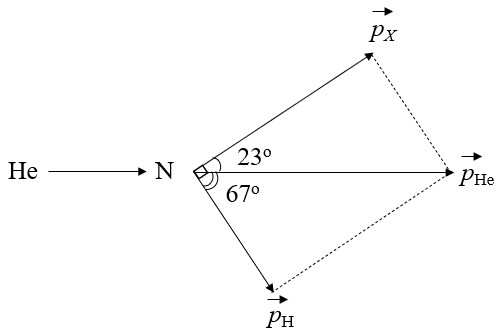
\includegraphics[scale=0.8]{../figs/VN12-PH-47-L-028-2-H2.jpg}
		\end{center}
		
		Phương trình phản ứng
		\begin{equation*}
			^4_2\text{He} + ^{14}_{\ 7}\text{N}\ \rightarrow ^{14}_{\ 8} X + ^1_1\text{H}.
		\end{equation*}
		
		Áp dụng định luật bảo toàn động lượng
		\begin{equation*}
			\vec{p}_X=\vec{p}_\text{He}+\vec{p}_\text{H}.
		\end{equation*}
		
		Áp dụng định lý hàm sin
		\begin{equation*}
			\dfrac{p_\text{He}}{\sin 90^\circ}=\dfrac{p_\text{H}}{\sin 23^\circ}=\dfrac{p_X}{\sin 67^\circ}
		\end{equation*}
		\begin{equation*}
			\Rightarrow
			\left\{\begin{array}{ll}{p_\text{He}=\dfrac{\sin 90^\circ}{\sin 67^\circ}{p_X}}&\\
				{p_\text{H}=\dfrac{\sin 23^\circ}{\sin 67^\circ}{p_X}}&\end{array}\right.
		\end{equation*}
		\begin{equation*}
			\Rightarrow\left\{\begin{array}{ll}{p_\text{He}=1,086p_X}&\\{p_\text{H}^{2}=0,424p_X}&\end{array}\right.
		\end{equation*}
		\begin{equation*}
			\Rightarrow\left\{\begin{array}{ll}{p_\text{He}^{2}=1,18p_X^2}&\\{p_\text{H}^{2}=0,18p_X^2}&\end{array}\right.
		\end{equation*}
		\begin{equation*}
			\Rightarrow \left\{\begin{array}{ll}{2{m_\text{He}}{W_\textrm{đ He}}=1,18\cdot2{m_X}{W_\textrm{đ X}}}&\\
				{2{m_\text{H}}{W_\textrm{đ H}}=0,18\cdot2{m_X}{W_\textrm{đ X}}}&\end{array}\right.
		\end{equation*}
		\begin{equation*}
			\Rightarrow \left\{\begin{array}{ll}{{W_\textrm{đ He}}=5,015W_{\textrm{đ }X}}&\\
				{{W_\textrm{đ H}}=3,06W_{\textrm{đ }X}}.&\end{array}\right.
		\end{equation*}
		
		
		Áp dụng định luật bảo toàn năng lượng
		\begin{equation*}
			W_\textrm{đ He} - \SI{1,21}{\mega\electronvolt}= W_{\textrm{đ }X} + W_\textrm{đ H}
		\end{equation*}
		\begin{equation*}
			\Rightarrow 5,015W_{\textrm{đ }X} - \SI{1,21}{\mega\electronvolt} = W_{\textrm{đ }X} + 3,06W_{\textrm{đ }X}
		\end{equation*}
		\begin{equation*}
			\Rightarrow W_{\textrm{đ }X}=\SI{1,27}{\mega\electronvolt}.
		\end{equation*}
		
		\begin{center}
			\textbf{Câu hỏi tương tự}
		\end{center}
		Bắn phá một proton vào hạt nhân $ ^{7}_{3} \text{Li} $ đang đứng yên. Phản ứng hạt nhân sinh ra hai hạt nhân $ X $ giống nhau và có cùng tốc độ. Biết tốc độ của proton bằng $ 4 $ lần tốc độ của hạt nhân $ X $. Coi khối lượng của hạt nhân bằng số khối theo đơn vị $ u $. Góc tạo bởi phương chuyển động của hai hạt $ X $ là 
		\begin{mcq}(4)
			\item $ 60^\circ $.	
			\item $ 90^\circ $.	
			\item $ 120^\circ $.	
			\item $ 150^\circ $.		
		\end{mcq}
		
		\textbf{Đáp án:} C.
	}
	
\end{dang}

\section{Bài tập tự luyện}
\begin{enumerate}[label=\bfseries Câu \arabic*:]
	\item \mkstar{1} [4]
	\cauhoi
	{Trong phản ứng hạt nhân, đại lượng không bảo toàn là
		\begin{mcq}(4)
			\item động lượng.
			\item số nuclon.
			\item điện tích.
			\item khối lượng.
		\end{mcq}
	}
	
	\loigiai
	{		\textbf{Đáp án: D.}
		
		Trong phản ứng hạt nhân, khối lượng không được bảo toàn (tổng khối lượng các hạt trước và sau phản ứng không bằng nhau).
		
	}
	\item \mkstar{1} [7]
	\cauhoi
	{Trong một phản ứng hạt nhân, có sự bảo toàn
		\begin{mcq}(4)
			\item số nuclon.
			\item số proton.
			\item số nơtron.
			\item khối lượng.
		\end{mcq}
	}
	
	\loigiai
	{		\textbf{Đáp án: A.}
		
		Trong một phản ứng hạt nhân, có sự bảo toàn số nuclon (cũng là số khối).
		
		Chú ý rằng trong một phản ứng hạt nhân, có sự bảo toàn điện tích, nhưng không bảo toàn số proton.
		
	}
	\item \mkstar{2} [13]
	\cauhoi
	{Proton có động năng $W_{\text{đ} \ce{p}} = \SI{5.0}{MeV}$ được bắn vào $\ce{^9_4 Be}$ nằm yên. Phản ứng hạt nhân sinh ra $\ce{^4_2 He}$ và $\ce{^A_Z X}$. Sau phản ứng hạt nhân $\ce{^4_2 He}$ có động năng $W_{\text{đ} \ce{He}} = \SI{4.1}{MeV}$ và vận tốc $\vec v_{\ce{He}}$ vuông góc với vận tốc $\vec v_{\ce{p}}$ lúc đầu. Tính động năng $W_{\text{đ} \ce{X}}$ của hạt nhân X.
		\begin{mcq}(4)
			\item $\SI{3.57}{MeV}$.
			\item $\SI{7.40}{MeV}$.
			\item $\SI{9.10}{MeV}$.
			\item $\SI{0.90}{MeV}$.
		\end{mcq}
	}
	
	\loigiai
	{		\textbf{Đáp án: A.}
		
		Phương trình phản ứng:
		$$\ce{^1_1 p} + \ce{^9_4 Be} \longrightarrow \ce{^4_2 He} + \ce{^6_3 X}.$$
		
		Áp dụng định luật bảo toàn động lượng cho các hạt trước và sau phản ứng:
		$$\vec p_{\ce{\alpha}} = \vec p_{\ce{p}} + \vec p_{\ce{O}}$$
		
		Hình vẽ minh họa:
		\begin{center}
			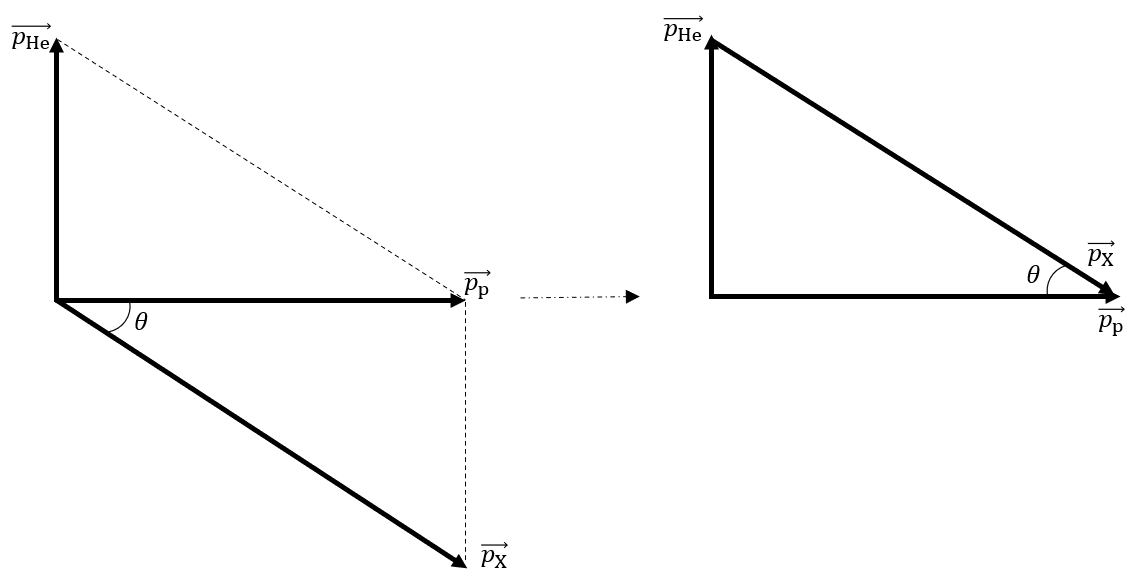
\includegraphics[scale=0.8]{../figs/VN12-2021-PH-TP037-3}
		\end{center}
		
		Áp dụng định lý Py-ta-go:
		$$p_{\ce{X}}^2 = p_{\ce{He}}^2 + p_{\ce{p}}^2$$
		
		Với $p^2=2mK$, ta được:
		$$2 m_{\ce{X}} K_{\ce{X}} = 2 m_{\ce{He}} K_{\ce{He}} +  2 m_{\ce{p}} K_{\ce{p}} $$
		
		Giải phương trình, tìm được:
		$$K_{\ce{X}} = \SI{3.57}{MeV}$$
		
	}
	
	\item \mkstar{2} [7]
	\cauhoi
	{Cho phản ứng hạt nhân sau:
		$$\ce{^9_4 Be} + \ce{p} \longrightarrow \ce{X} + \ce{^6_3 Li}$$
		
		Biết $m_{\ce{Be}} = \SI{9.01219}{u}$, $m_{\ce{p}} = \SI{1.00783}{u}$, $m_{\ce{X}} = \SI{4.00620}{u}$, $m_{\ce{Li}} = \SI{6.01515}{u}$, $\SI{1}{u} = \SI{931}{MeV/c^2}$. Cho hạt $\ce{p}$ có động năng $K_{\ce{p}} = \SI{5.45}{MeV}$ bắn phá hạt nhân $\ce{Be}$ đứng yên, hạt nhân $\ce{Li}$ bay ra với động năng $\SI{3.55}{MeV}$. Động năng của hạt $\ce{X}$ bay ra có giá trị là
		\begin{mcq}(4)
			\item $\SI{0.66}{MeV}$.
			\item $\SI{0.66}{eV}$.
			\item $\SI{66}{MeV}$.
			\item $\SI{660}{eV}$.
		\end{mcq}
	}
	
	\loigiai
	{		\textbf{Đáp án: A.}
		
		Năng lượng tỏa ra hoặc thu vào của phản ứng:
		$$Q=(m_\text{t} - m_\text{s})c^2 = \SI{-1.23823}{MeV}$$
		
		Lại có $Q=K_{\text{s}} - K_{\text{t}} = K_{\ce{X}} + K_{\ce{Li}} - K_{\ce{p}} \Rightarrow K_{\ce{X}} = \SI{0.66}{MeV}$
		
	}
	\item \mkstar{3} [1]
	\cauhoi
	{Người ta dùng hạt $\ce{\alpha}$ có động năng $K_{\ce{\alpha}}$ bắn vào hạt nhân nhôm $\ce{^27_13 Al}$ đứng yên gây ra phản ứng 
		$$\ce{^4_2 He} + \ce{^27_13 Al} \longrightarrow \ce{^30_15 P} + \ce{^1_0 n}$$
		Biết hạt nơtron và hạt nhân $\ce{^30_15 P}$ sinh ra sau phản ứng có động năng lần lượt là $\SI{1.8}{MeV}$ và $\SI{1}{MeV}$. Biết khối lượng của các hạt lần lượt là $m_{\ce{\alpha}} = \SI{4.00151}{u}$; $m_{\ce{Al}} = \SI{26.97435}{u}$; $m_{\ce{P}} = \SI{29.97005}{u}$; $m_{\ce{n}} = \SI{1.00867}{u}$. Động năng hạt $\ce{\alpha}$ là $K_{\ce{\alpha}}$ bằng
		\begin{mcq}(4)
			\item $\SI{5.464}{MeV}$.
			\item $\SI{4.232}{MeV}$.
			\item $\SI{5.644}{MeV}$.
			\item $\SI{4.328}{MeV}$.
		\end{mcq}
	}
	
	\loigiai
	{		\textbf{Đáp án: A.}
		
		Ta có năng lượng tỏa ra hoặc thu vào từ phản ứng là
		$$Q=(m_\text{t} - m_\text{s})c^2 = \SI{-2.66409}{MeV}$$
		
		Mà $Q=K_\text{s} - K_\text{t} \Rightarrow K_{\ce{P}} + K_{\ce{n}} - K_{\ce{\alpha}} - K_{\ce{Al}} = \SI{-2.66409}{MeV}$, suy ra $K_{\ce{\alpha}} = \SI{5.464}{MeV}$. (Chú ý rằng $K_{\ce{Al}}=0$ vì hạt nhân nhôm đứng yên)
	}
	\item \mkstar{3} [4]
	\cauhoi
	{Dùng một hạt $\ce{\alpha}$ có động năng $\SI{7.7}{MeV}$ bắn vào hạt nhân $\ce{^14_7 N}$ đang đứng yên gây ra phản ứng
		$$\ce{^4_2 He} + \ce{^14_7 N} \longrightarrow \ce{^1_1 p} + \ce{^17_8 O}$$
		Hạt proton bay ra theo phương vuông góc với phương bay tới của hạt $\ce{^4_2 He}$. Cho khối lượng các hạt nhân: $m_{\ce He} = \SI{4.0015}{u}$, $m_{\ce{N 14}} = \SI{13.9992}{u}$, $m_{\ce{O 17}} = \SI{16.9947}{u}$, $m_{\ce{p}} = \SI{1.0073}{u}$. Động năng của hạt nhân $\ce{^17_8 O}$ là
		\begin{mcq}(4)
			\item $\SI{2.075}{MeV}$.
			\item $\SI{2.214}{MeV}$.
			\item $\SI{6.145}{MeV}$.
			\item $\SI{1.345}{MeV}$.
		\end{mcq}
	}
	
	\loigiai
	{		\textbf{Đáp án: A.}
		
		
		Áp dụng định luật bảo toàn động lượng cho các hạt trước và sau phản ứng:
		$$\vec p_{\ce{\alpha}} = \vec p_{\ce{p}} + \vec p_{\ce{O}}$$
		
		Hình vẽ minh họa:
		\begin{center}
			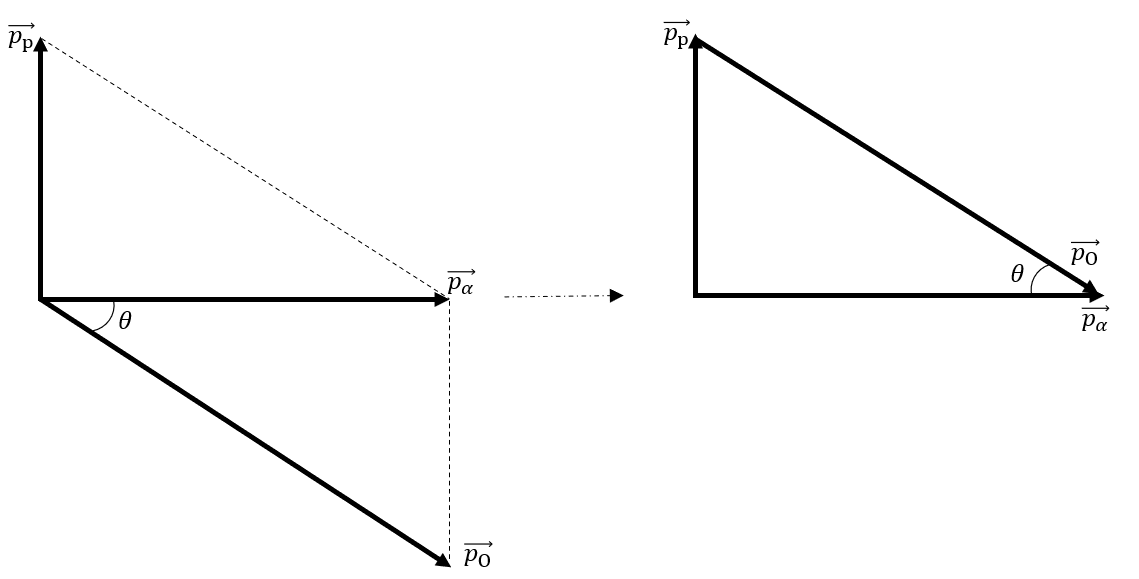
\includegraphics[scale=0.8]{../figs/VN12-2021-PH-TP037-2}
		\end{center}
		
		Áp dụng định lý Py-ta-go:
		$$p_{\ce{O}}^2 = p_{\ce{\alpha}}^2 + p_{\ce{p}}^2$$
		
		Với $p^2=2mK$, ta được:
		$$2 m_{\ce{O}} K_{\ce{O}} = 2 m_{\ce{\alpha}} K_{\ce{\alpha}} +  2 m_{\ce{p}} K_{\ce{p}} $$
		
		Kết hợp với công thức tính năng lượng tỏa ra hoặc thu vào:
		$$Q=(m_{\text{t}} - m_{\text{s}})c^2 = \SI{-1.21095}{MeV} = K_{\text s} - K_{\text t} = K_{\ce{p}} + K_{\ce{O}} - K_{\ce{He}}$$
		
		Giải hệ 2 phương trình, tìm được:
		$K_{\ce{p}} = \SI{4.417}{MeV}$ và $K_{\ce{O}} = \SI{2.072}{MeV}$
		
		Động năng của hạt nhân $\ce{^17_8 O}$ là xấp xỉ $\SI{2.075}{MeV}$.
	}
	\item \mkstar{3} [12]
	\cauhoi
	{Hạt nhân $\ce{^222_86 Rn}$ phóng xạ $\alpha$ tạo thành hạt nhân X. Ban đầu, hạt nhân $\ce{^222_86 Rn}$ đứng yên. Khối lượng mỗi hạt nhân bằng số khối của nó (đơn vị u). Ngay sau khi tạo thành, hạt $\ce{\alpha}$ và hạt X có tốc độ lần lượt là $v_1=\SI{2e7}{m/s}$ và $v_2$. Giá trị của $v_2$ xấp xỉ bằng
		\begin{mcq}(2)
			\item $\SI{366.972e3}{m/s}$.
			\item $\SI{10.034e5}{m/s}$.
			\item $\SI{109.021e3}{m/s}$.
			\item $\SI{605.015e3}{m/s}$.
		\end{mcq}
	}
	
	\loigiai
	{		\textbf{Đáp án: A.}
		
		Phản ứng hạt nhân:
		$$\ce{^222_86 Rn} \longrightarrow \ce{^4_2 He} + \ce{^218_84 X}$$
		
		Áp dụng định luật bảo toàn động lượng cho các hạt trước và sau phản ứng:
		$$\vec p_{\ce{Rn}} = \vec p_{\ce{\alpha}} + \vec p_{\ce{X}}$$
		
		Do $\vec p_{\ce{Rn}} = 0$ nên $\vec p_{\ce{\alpha}} + \vec p_{\ce{X}}$, suy ra:
		$$p_{\ce{\alpha}} = p_{\ce{X}}$$
		
		Với $p=\sqrt{2mK}$, và $\SI{1}{u} = \SI{1.6605e-27}{kg}$ ta được:
		$$2 m_{\ce{\alpha}} K_{\ce{\alpha}} = 2 m_{\ce{X}} K_{\ce{X}} \Rightarrow v_{\ce{X}} = \SI{366.972e3}{m/s}$$
	}
	\item \mkstar{4} [2]
	\cauhoi
	{Bắn một hạt proton có khối lượng $m_{\ce{H}}$ vào hạt nhân $\ce{^7_3 Li}$ đứng yên. Phản ứng tạo ra hai hạt nhân X giống nhau bay ra với vận tốc có cùng độ lớn và có phương vuông góc với nhau. Nếu xem gần đúng khối lượng hạt nhân theo đơn vị u bằng số khối của nó thì tỉ số tốc độ $v'$ của hạt X và $v$ của hạt proton là
		\begin{mcq}(4)
			\item $\dfrac{v'}{v} = \dfrac{1}{4}$.
			\item $\dfrac{v'}{v} = \dfrac{\sqrt{2}}{4}$.
			\item $\dfrac{v'}{v} = \dfrac{\sqrt 2}{8}$.
			\item $\dfrac{v'}{v} = \dfrac{1}{2}$.
		\end{mcq}
	}
	
	\loigiai
	{		\textbf{Đáp án: C.}
		
		Áp dụng định luật bảo toàn động lượng cho các hạt trước và sau phản ứng:
		$$\vec p_{\text t} = \vec p_{\text s} \Rightarrow p_{\ce{p}}^2 = p_{\ce{X}}^2 + p_{\ce{X}}^2 = 2p_{\ce{X}}^2$$
		
		Mà theo liên hệ $p^2=2mK$, suy ra:
		$$2 m_{\ce{p}} K_{\ce{p}} = 2 \cdot 2 m_{\ce{X}} K_{\ce{X}} \Rightarrow m_{\ce{p}} K_{\ce{p}} = 2 m_{\ce{X}} K_{\ce{X}}$$
		
		Thay $K=\dfrac{1}{2} mv^2$, ta được:
		$$m_{\ce{p}} \cdot \dfrac{1}{2} m_{\ce{p}} v_{\ce{p}}^2 = 2 m_{\ce{X}} \cdot \dfrac{1}{2} m_{\ce{X}} v_{\ce{X}}^2 \Rightarrow \dfrac{v_{\ce{X}}^2}{v_{\ce{p}}^2} = \dfrac{m_{\ce{p}}^2}{2 m_{\ce{X}}^2} = \dfrac{1^2}{2 \cdot 4^2} = \dfrac{1}{32} \Rightarrow \dfrac{v'}{v} = \sqrt{\dfrac{1}{32}} = \dfrac{\sqrt 2}{8}$$
		
	}
	
	\item \mkstar{4} [3]
	\cauhoi
	{Bắn hạt nơtron có động năng $\SI{2}{MeV}$ vào hạt nhân $\ce{^6_3 Li}$ đứng yên gây ra phản ứng
		$$\ce{^1_0 n} + \ce{^6_3 Li} \longrightarrow \ce{X} + \ce{\alpha}.$$
		Hạt $\ce{\alpha}$ và hạt nhân $\ce{X}$ bay ra theo các hướng hợp với hướng tới của nơtron những góc tương ứng bằng $\theta = 15^\circ$ và $\varphi = 30^\circ$. Lấy tỉ số giữa các khối lượng hạt nhân bằng tỉ số giữa các số khối của chúng. Bỏ qua bức xạ gamma. Năng lượng của phản ứng hạt nhân \textbf{gần với giá trị nào nhất?}
		\begin{mcq}(4)
			\item Tỏa $\SI{1.52}{MeV}$.
			\item Thu $\SI{1.66}{MeV}$. 
			\item Thu $\SI{1.52}{MeV}$.
			\item Tỏa $\SI{1.66}{MeV}$.
		\end{mcq}
	}
	
	\loigiai
	{		\textbf{Đáp án: B.}
		
		Áp dụng định luật bảo toàn động lượng cho các hạt trước và sau phản ứng:
		$$\vec p_{\ce{n}} = \vec p_{\ce{X}} + \vec p_{\ce{\alpha}}$$
		
		Hình vẽ minh họa:
		\begin{center}
			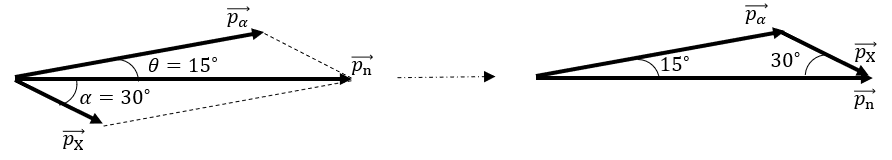
\includegraphics{../figs/VN12-2021-PH-TP037-1}
		\end{center}
		
		Áp dụng định lý hàm số sin:
		$$\dfrac{p_{\ce{n}}}{\sin 135^\circ} = \dfrac{p_{\ce{\alpha}}}{\sin 30^\circ} = \dfrac{p_{\ce{X}}}{\sin 15^\circ}$$
		
		Với $p=\sqrt{2mK}$, ta được:
		$$\dfrac{p_{\ce{n}}}{\sin 135^\circ} = \dfrac{p_{\ce{\alpha}}}{\sin 30^\circ} \Rightarrow \dfrac{\sqrt{2 m_{\ce{n}} K_{\ce{n}}}}{\sin 135^\circ} = \dfrac{\sqrt{2 m_{\ce{\alpha}} K_{\ce{\alpha}}}}{\sin 30^\circ}\Rightarrow K_{\ce{\alpha}} = \SI{0.25}{MeV} $$
		
		$$\dfrac{p_{\ce{n}}}{\sin 135^\circ} = \dfrac{p_{\ce{X}}}{\sin 15^\circ} \Rightarrow \dfrac{\sqrt{2 m_{\ce{n}} K_{\ce{n}}}}{\sin 135^\circ} = \dfrac{\sqrt{2 m_{\ce{X}} K_{\ce{X}}}}{\sin 15^\circ}\Rightarrow K_{\ce{X}} = \SI{0.09}{MeV} $$
		
		Năng lượng tỏa ra hoặc thu vào:
		$$Q=K_{\text{s}} - K_{\text{t}} = \SI{-1.66}{MeV}$$
		
		Do $Q<0$ nên phản ứng thu năng lượng.
	}
	
	\item \mkstar{2} [4]
	\cauhoi
	{Cho phản ứng hạt nhân $\ce{^4_2 He} + \ce{^27_13 Al} \longrightarrow \ce{^30_15 P} + \ce{n}$, khối lượng của các hạt nhân là $m_{\ce{He}} = \SI{4.0015}{u}$, $m_{\ce{Al}} = \SI{26.97435}{u}$, $m_{\ce{P}} = \SI{29.97005}{u}$, $m_{\ce{n}} = \SI{1.00867}{u}$, $\SI{1}{u} = \SI{931.5}{MeV/c^2}$. Năng lượng mà phản ứng này tỏa ra hoặc thu vào là bao nhiêu?
		\begin{mcq}(2)
			\item Tỏa ra $\SI{5.022648}{MeV}$.
			\item Tỏa ra $\SI{5.022648e-13}{J}$.
			\item Thu vào $\SI{2.673405}{MeV}$.
			\item Thu vào $\SI{2.673405e-13}{J}$.
		\end{mcq}
	}
	
	\loigiai
	{		\textbf{Đáp án: C.}
		
		Năng lượng tỏa ra hoặc thu vào:
		$$Q=(m_{\text{t}} - m_\text{s}) c^2 = \SI{-2.673405}{MeV}$$
		
		Vì $Q<0$ nên phản ứng thu năng lượng.
		
	}
	
	\item \mkstar{2} [2]
	\cauhoi
	{Cho phản ứng hạt nhân $\ce{^55_25 Mn} + \ce{p} \longrightarrow \ce{^55_26 Fe} + \ce{n}$, khối lượng của các hạt nhân là $m_{\ce{Mn}} = \SI{54.9381}{u}$, $m_{\ce{Fe}} = \SI{54.9380}{u}$, $m_{\ce{p}} = \SI{1.0073}{u}$, $m_{\ce{n}} = \SI{1.0087}{u}$, $\SI{1}{u} = \SI{931.5}{MeV/c^2}$. Phản ứng trên
		\begin{mcq}(2)
			\item tỏa năng lượng $\SI{12.1095}{MeV}$.
			\item tỏa năng lượng $\SI{1.21095}{MeV}$.
			\item thu năng lượng $\SI{12.1095}{MeV}$.
			\item thu năng lượng $\SI{1.21095}{MeV}$.
		\end{mcq}
	}
	
	\loigiai
	{		\textbf{Đáp án: D.}
		
		Năng lượng tỏa ra hoặc thu vào:
		$$Q=(m_{\text{t}} - m_\text{s}) c^2 = \SI{-1.21095}{MeV}$$
		
		Vì $Q<0$ nên phản ứng thu năng lượng.
		
	}
	\item \mkstar{2} [2]
	\cauhoi
	{Giả sử trong một phản ứng hạt nhân, tổng khối lương hai hạt trước phản ứng lớn hơn tổng khối lượng hai hạt sau phản ứng là $\SI{0.02}{u}$. Cho $\SI{1}{u} = \SI{931.5}{MeV/c^2}$. Phản ứng hạt nhân này
		\begin{mcq}(2)
			\item tỏa năng lượng $\SI{1.863}{MeV}$.
			\item thu năng lượng $\SI{1.863}{MeV}$.
			\item tỏa năng lượng $\SI{18.63}{MeV}$.
			\item thu năng lượng $\SI{18.63}{MeV}$.
		\end{mcq}
	}
	
	\loigiai
	{		\textbf{Đáp án: C.}
		
		Vì $m_{\text{t}}>m_{\text{s}}$ nên phản ứng hạt nhân tỏa năng lượng:
		
		Năng lượng tỏa ra:
		$$Q=(m_{\text{t}} - m_\text{s}) c^2 = \SI{18.63}{MeV}$$
		
	}
	
	\item \mkstar{2} [3]
	\cauhoi
	{Cho phản ứng hạt nhân $\ce{^23_11 Na} + \ce{^1_1 H} \longrightarrow \ce{^4_2 He} + \ce{^20_10 Ne}$. Lấy khối lượng của các hạt nhân $\ce{^23_11 Na}$, $\ce{^20_10 Ne}$, $\ce{^4_2 He}$, $\ce{^1_1 H}$ lần lượt là $\SI{22.9837}{u}$, $\SI{19.9869}{u}$, $\SI{4.0015}{u}$, $\SI{1.0073}{u}$ và $\SI{1}{u} = \SI{931.5}{MeV/c^2}$. Năng lượng của phản ứng này
		\begin{mcq}(2)
			\item thu vào $\SI{2.4219}{MeV}$.
			\item thu vào $\SI{3.4524}{MeV}$.
			\item tỏa ra $\SI{3.4524}{MeV}$.
			\item tỏa ra $\SI{2.4219}{MeV}$.
		\end{mcq}
	}
	
	\loigiai
	{		\textbf{Đáp án: D.}
		
		Năng lượng tỏa ra hoặc thu vào:
		$$Q=(m_{\text{t}} - m_\text{s}) c^2 = \SI{2.4219}{MeV}$$
		
		Vì $Q>0$ nên phản ứng tỏa năng lượng.
	}
	\item \mkstar{2} [9]
	\cauhoi
	{Xét một phản ứng hạt nhân $\ce{^2_1 H} + \ce{^2_1 H} \longrightarrow \ce{^3_2 He} + \ce{^1_0 n}$. Biết $m_{\ce{H}} = \SI{2.0135}{u}$, $m_{\ce{He}} = \SI{3.0149}{u}$, $m_{\ce{n}} = \SI{1.0087}{u}$, lấy $\SI{1}{u} = \SI{931.5}{MeV/c^2}$. Phản ứng trên
		\begin{mcq}(2)
			\item tỏa năng lượng $\SI{3.1671}{MeV}$.
			\item thu năng lượng $\SI{3.1671}{MeV}$.
			\item tỏa năng lượng $\SI{6.0371}{MeV}$.
			\item thu năng lượng $\SI{6.0371}{MeV}$.
		\end{mcq}
	}
	
	\loigiai
	{		\textbf{Đáp án: A.}
		
		Năng lượng tỏa ra hoặc thu vào:
		$$Q=(m_{\text{t}} - m_\text{s}) c^2 = \SI{3.1671}{MeV}$$
		
		Vì $Q>0$ nên phản ứng tỏa năng lượng.
	}

	\item \mkstar{2} 
	\cauhoi
	{Cho phản ứng hạt nhân sau $\ce{^2_1 H} + \ce{^2_1 Be} \longrightarrow \ce{^3_2 He} + X + \SI{2,1}{MeV}$. Năng lượng tỏa ra từ phản ứng trên khi tổng hợp được $\SI{4}{g}$ Heli bằng
		
		\begin{mcq}(2)
			\item $\text{5,61}\cdot 10^{24}\ \text{MeV}$.
			\item $\text{1,26}\cdot 10^{24}\ \text{MeV}$.
			\item $\text{5,06}\cdot 10^{24}\ \text{MeV}$.
			\item $\text{5,61}\cdot 10^{23}\ \text{MeV}$.
		\end{mcq}
	}
	
	\loigiai
	{		\textbf{Đáp án: B.}
		
	$$\Delta E = nW_\text{lk} = \dfrac{m}{4}N_A W_\text{lk} = \text{1,26}\cdot 10^{24}\ \text{MeV}.$$
	}
	
		\item \mkstar{2} 
	\cauhoi
	{Phân hạch hạt nhân $\ce{^{235} U}$ trong lò phản ứng sẽ tỏa ra năng lượng $\SI{200}{MeV}$. Nếu phân hạch $\SI{1}{g}$ $\ce{^{235} U}$thì năng lượng tỏa ra bằng bao nhiêu. Cho $N_A = \text{6,02}\cdot 10^{23}\ \text{mol}^{-1}$.
		
		\begin{mcq}(2)
			\item $\text{5,013}\cdot 10^{25}\ \text{MeV}$.
			\item $\text{5,123}\cdot 10^{23}\ \text{MeV}$.
			\item $\text{5,123}\cdot 10^{24}\ \text{MeV}$.
			\item $\text{5,123}\cdot 10^{25}\ \text{MeV}$.
		\end{mcq}
	}
	
	\loigiai
	{		\textbf{Đáp án: B.}
		
		$$\Delta E = nW_\text{lk} = \dfrac{m}{235}N_A W_\text{lk} = \text{5,123}\cdot 10^{23}\ \text{MeV}.$$
	}
	
	
\end{enumerate}

